\documentclass[11pt]{elsarticle}

% ---------------------------------------------------------------
%                 PACKAGES  (minimum set)
% ---------------------------------------------------------------
\usepackage[T1]{fontenc}
\usepackage[utf8]{inputenc}
\usepackage{lmodern}            % high-quality Latin Modern fonts
\usepackage{ltablex}
\usepackage{setspace}\onehalfspacing     % 1.5 line spacing
\usepackage{amsmath,amssymb,mathtools}
\usepackage{graphicx}
\usepackage{booktabs,multirow}
\usepackage{hyperref}
\usepackage{enumitem}
\setlist{nosep}
\usepackage{caption,subcaption}
\usepackage{float}
\usepackage{booktabs}     % professional horizontal rules
\usepackage{multirow}     % for \multirow
\usepackage{tabularx}     % width-responsive tables
\usepackage{threeparttable}
\usepackage{multicol}

\usepackage{algorithm} \usepackage{algpseudocode}

% Smart, journal-style cross-references
\usepackage[capitalize,noabbrev,nameinlink]{cleveref}

% Always call anything below a section simply “Section”
\crefname{section}{Section}{Sections}
\Crefname{section}{Section}{Sections}
\crefname{subsection}{Section}{Sections}
\Crefname{subsection}{Section}{Sections}
\crefname{subsubsection}{Section}{Sections}
\Crefname{subsubsection}{Section}{Sections}
\crefname{paragraph}{Section}{Sections}      % in case you ever label a \paragraph
\Crefname{paragraph}{Section}{Sections}


\captionsetup[algorithm]{labelformat=empty}     % for [H]
\biboptions{authoryear,round,sort&compress}



\makeatletter
\renewcommand\paragraph{\@startsection{paragraph}{4}{\z@}
  {3.25ex \@plus1ex \@minus.2ex}
  {-1em}
  {\normalfont\normalsize\itshape}}
\makeatother

\setcounter{secnumdepth}{3}
\setcounter{tocdepth}{2}   

% ---------------------------------------------------------------
%              FRONT MATTER
% ---------------------------------------------------------------
\journal{Computers \& Industrial Engineering}



\begin{document}
\begin{frontmatter}

\title{Efficient and Practical Solutions for Correlated Storage Location Assignment Problem in Automated Warehouse Environment}

\begin{abstract}
Warehouse operations strongly shape supply-chain effectiveness. We study the Correlated Storage Location Assignment Problem, which is a cornerstone problem of modern warehousing challenges, focusing on optimizing product placement to streamline order preparation processes. This paper introduces an innovative approach to the Correlated Storage Location Assignment Problem that departs from the conventional emphasis on minimizing travel distance within warehouses. Specifically, our objective is to minimize the total number of stations visited by all orders during preparation, thus enhancing operational efficiency and reducing global preparation time.
\end{abstract}

\begin{keyword}
Warehouse optimization \sep Integer programming \sep Heuristics \sep Column generation \sep Logistics
\end{keyword}

\end{frontmatter}
\clearpage


\section{Introduction}

Efficient warehouse operations significantly influence the performance of supply chains. Order picking alone typically accounts for 50--65\% of warehouse operating costs \cite{xie2024combi}, making optimized storage assignment crucial. Central to this optimization challenge is the Correlated Storage Location Assignment Problem (CSLAP), which focuses on strategically placing products to streamline order preparation and fulfillment.

Traditional CSLAP models primarily aim to \emph{minimize travel distance} during order preparation \cite{islam2023}. However, in automated or conveyor-driven picking systems, \emph{reducing the number of station stops} is also critical. Each additional conveyor stop introduces waiting times, queuing delays, and extra operator handling, significantly impacting overall throughput. By explicitly targeting station-stop reduction, our approach addresses this often-overlooked dimension, minimizing congestion and accelerating fulfillment processes.

We propose three methods to tackle CSLAP: (i) a heuristic clustering approach that groups frequently co-ordered products and assigns them to stations, (ii) A mixed-integer linear program (MILP) that minimizes station visits while enforcing a balanced workload for each station in the warehouse, and (iii) a Column Generation (CG) framework that decomposes CSLAP into a master problem selecting optimal product-station assignment patterns, alongside multiple pricing subproblems generating feasible patterns for each station. 

Recognizing that established facilities cannot afford large, disruptive re-slotting waves, we extend the MILP with a \emph{limited-reassignment} mechanism that explicitly trades off the benefit of fewer station visits against the operational cost of moving products \citep{chabot2024reassignment}. This enables a \emph{continuous-improvement} rollout: warehouses re-slot a manageable subset in each cycle, harvest measurable throughput gains, and iterate, all without interrupting daily operations.

The broader contribution of our research is to bridge the gap between elegant but small-scale algorithms in the literature and the realities of large, automated warehouses. We show how core operations research technics like heuristics, constraint programming along with objective optimization, and decomposition via column generation—can be combined into solution approaches that are \emph{both} theoretically sound and industrially scalable. In doing so, we turn correlated storage assignment from a compelling modeling concept into a practical tool for large-scale order preparation, aligning scientific optimality with day-to-day implement ability.
%This work largely extends preliminary results presented earlier in a peer-reviewed conference paper \citep{ErmalBelul2025}.
This work largely extends preliminary results presented earlier in a peer-reviewed conference paper, details are withheld for double anonymized review and will be reinstated after acceptance.

\noindent
% \textbf{Organization.} Section~\ref{sec:case_study} describes the case and metrics. Section~\ref{sec:solution_approaches} details our proposed solution approaches: Heuristic, MILP, CG and reports results, including robustness tests. Section~\ref{sec:limited_reassignment} covers the limited-reassignment extension. Section~\ref{sec:conclusion} discusses implications and future work.



\section{Case Study}\label{sec:case_study}

Our case study examines the Correlated Storage Location Assignment Problem (CSLAP) on a real-world instance using historical data provided by Company A, which operates an automated warehouse. The initial placement of products $(P)$ within this warehouse was arranged in the best possible way by operators, drawing upon their extensive practical knowledge and daily operational expertise. \\
\begin{figure}[H]
\centering

\includegraphics[width=0.9\linewidth]{Images_CSLAP/GARE_ZOOM001_compressed.png}
\caption{Picking Section Illustration}
\end{figure}

The system is organized around a main conveyor along which orders advance in sequence. Branch lines off the main conveyor correspond to individual picking stations $(S)$. At each station $(s \in S)$, an order ($o \in O$) temporarily leaves the main conveyor so that human pickers can retrieve the required items from nearby shelving and place them into the order bin. After the station’s items are collected, the bin returns to the main conveyor and proceeds its journey. This process repeats at subsequent stations until all items in the order $(P_o)$ are collected. Finally, the completed bin exits through the main conveyor output, ready for dispatch.

In this setting, limiting the number of station stops per order is essential, since each stop significantly contributes to the total order preparation time due to waiting and queuing at the stations. Our aim is to demonstrate effectiveness under operational conditions in an actual warehouse. We make use of some historical data from Company A (with $|P|=21\,877$, $|O|=284\,871$, and $|S|=26$).
Because our dataset records, for every order, the \textit{order ID}, the corresponding \textit{product IDs}, the current \textit{station ID}, and the overall \textit{number of pick locations available at each station}, we model CSLAP at the station level rather than at the level of individual storage slots. We make the practical assumption that each station’s internal shelving is \emph{modular}: dividers can be rearranged without altering the station’s \emph{total} storage capacity.  This intra-station flexibility allows us to concentrate on the key decision, ­\emph{which products $(p \in P)$ should share the same station}, without being restricted by fixed slot geometries. 
Throughout our analysis, the global capacity constraint (total number of locations per station) is strictly respected, even though the internal configuration of those locations may be rebalanced.

\subsection{Evaluation Metrics}

We evaluate against the company’s original assignment using: \\
\textbf{(1) Number of orders per number of visited Stations:} Illustrates for each possible number of visited stations the number of orders which has visited exactly this number of stations. \\
\textbf{(2) Number of Lines Per Station:} 
Assesses workload distribution by quantifying the number of retrieval lines (instances of product picking without considering quantity) per station. Additionally, we illustrate the \textit{relative change} in workload compared to the company's original assignment, computed as:
\begin{equation*}
        \text{Relative Change (\%)} = \frac{T_s' - T_s}{T_s} \times 100
\end{equation*}
where $T_s'$ denotes the number of pick-lines based on our assignment, and $T_s$ denotes the number of pick-lines in the original assignment of Company A at station $s$. 
This percentage highlights how significantly each station’s workload is impacted relative to its original assignment, providing insight into practical operational shifts while achieving our objective.
\subsection{Balanced-Workload Consideration: }\label{par:balanced_workload} Company A’s warehouse is \emph{heterogeneous}: stations differ markedly in both physical size and picker productivity. Some stations comprise many deep storage positions, obliging the operator to walk further to reach the rear slots; others are compact, with only a handful of easily accessible positions that can be serviced very quickly. Because of these structural differences, Company A has already tuned its layout so that labor demand, travel effort, and throughput are in equilibrium across stations. Preserving that equilibrium is essential for smooth day-to-day operations. Accordingly, our optimization seeks to minimize the number of station visits \emph{while allowing only minor deviations from the company’s pre-established workload profile $(T_s)$}. Throughout this paper, the term “balanced workload” therefore refers to a distribution that stays as close as practicable to Company A’s deliberately calibrated baseline, ensuring that no station becomes over- or under-utilized after re-slotting.



\begin{table}[htbp]
\centering
\small % reduce font size slightly to save more space
\begin{tabular}{cl}
\toprule
\textbf{Symbol} & \textbf{Definition}\\
\midrule
$P$ & set of products\\
$O$ & set of orders\\
$S$ & set of stations\\
$P_o$ & set of products requested in order $o \in O$\\
$\zeta_s$ & number of available storage locations at station $s \in S$\\
$L_p$ & total number of pick-lines for product $p \in P$ during the planning horizon\\
$T_s$ & number of pick-lines from the original assignment of Company A at $s \in S$\\
$V_s$ & processing speed at station $s \in S$ (lines/minute)\\
$K_s$ & set of feasible patterns (product assignments) for station $s \in S$\\

\bottomrule
\end{tabular}
\caption*{Summary of key notations}
\label{tab:notation}
\end{table}




\section{Literature Review}\label{sec:lit_review}
Our overview of CSLAP builds on the comprehensive systematic review by Islam and Uddin (2023) \cite{islam2023}. Their survey covers nearly thirty years of research, highlighting the evolution of solution strategies ranging from heuristic and meta-heuristic methods to data mining approaches. They underscore the critical role of strategic item placement in optimizing warehouse performance, emphasizing the challenge posed by the NP-hard nature of most CSLAP formulations.
Expanding on heuristic methods, \cite{trindade2022} introduced a two-phase heuristic clustering strategy that considered product correlations and additional constraints like product weight and precedence. This strategy achieved notable improvements in warehouse picking performance by reducing picker travel distances in real-world scenarios. \citet{zhang2019cie} introduced the \emph{demand correlation pattern} (DCP) to quantify item co-demand and embedded it into an optimization framework solved with metaheuristics, demonstrating substantial travel reductions on e-commerce data.\cite{wang2020} presented a data mining mechanism that uses order data without intermediate abstractions, improving picking performance compared with traditional popularity (ABC) or concept-driven pipelines. This approach seeks to minimize overall trip distance by carefully allocating storage according to item correlations, demonstrating the efficacy of data mining approaches in tackling CSLAP.

\cite{ansari2020} proposed a novel gravity model-based clustering heuristic inspired by Newton’s law of gravity. This method effectively grouped highly correlated products, substantially reducing the complexity of picker operations and enhancing operational efficiency.
Data-driven methodologies also gained prominence with \cite{pang2016}, who applied association-rule mining techniques to identify frequent product sets for storage assignment. This approach facilitated more efficient picker movements, validating the benefits of data-driven product assignment strategies.
 \cite{Egas2010-zb} introduced an iterative heuristic approach aimed at limiting the number of aisles traversed by an order picker, thereby decreasing travel time within the warehouse. Their approach, which arranges items using clustering analysis, significantly cuts down on journey time and distance, highlighting the role of item clustering in enhancing order-picking efficiency.

Recent work extends objectives beyond travel to human/robot co-working efficiency and surge handling. In robotic mobile fulfillment systems, \citet{zhang2023rmfs} formulated a bi-objective assignment balancing robots’ efficiency with human pickers’ energy expenditure. For e-commerce peaks, \citet{liu2023scattered} studied \emph{scattered storage} that intentionally disperses high-demand SKUs across multiple locations to parallelize picking and ease congestion. These lines of work highlight that storage design increasingly targets \emph{multiple} operational outcomes (time, congestion, ergonomics, resilience). 

A notable observation from the literature in both early and recent studies on CSLAP largely emphasized travel-distance minimization, our approach shifts the objective to \emph{station-visit minimization}. This objective is more closely aligned with operational bottlenecks in conveyor/zone systems, where each additional stop induces merge delays, queues, and extra handling.



\section{Solution Approaches}\label{sec:solution_approaches}

\subsection{First Approach: Heuristic Formulation}
Our initial approach to solve CSLAP was to develop a \emph{greedy-based algorithm} that could produce a near-optimal solution quickly. The method draws on graph-connectivity ideas \cite{west2001introduction} to build subsets of strongly co-occurring products that should be co-located at the same station. Using greedy selection with simple decision rules, we rank and include product pairs with the highest co-occurrence frequencies.


\subsubsection{Heuristic Approach: Greedy Product Clustering}

We partition the product set into “communities” of highly correlated items and then assign these communities to stations. Here, we will present some new notations to define different thresholds we have used for our heuristic process: 


\begin{itemize}
    \item \(\mathrm{MIN\_FREQ\_PREPROC}\): Defines the minimum frequency that a product appears, where \textbf{frequency} refers to how many distinct orders contain the product, independently of the ordered quantity.
    \item \(\mathrm{MIN\_FREQ}\): Minimum co-occurrence for pairs of products to be considered relevant.
    \item \(\mathrm{RATIO\_TO\_KEEP}\): Minimum fraction of co-occurrence relative to a product’s total frequency.
    \item \(\mathrm{MNOPPC}\): Maximum number of products allowed in a single community.
\end{itemize}

\noindent The core algorithm of our heuristic is:

\begin{algorithm}[H]
\caption{Algorithm 1: Greedy Product Clustering and Station Assignment (CSLAP)}
\label{alg:greedy-cslap}
\begin{algorithmic}[1]

\Statex \textbf{Step 1: Preprocessing and Pair Generation.}
\begin{enumerate}[label=(\alph*)]
\item Define $P^*=\{\,p\in P:\mathrm{freq}(p)\ge \mathrm{MIN\_FREQ\_PREPROC}\,\}$.
\item For each multi-item order $o\in O$, generate all unordered pairs $(p_i,p_j)$ with $p_i,p_j\in P^*$ and $i<j$.
\item Compute the co-occurrence count : \(\mathrm{count_{ij}} = \big|\{\,o \in O : \{p_i,p_j\} \subset o | i < j \}\big|, \)
and keep only pairs with $\mathrm{count}_{ij}\ge \mathrm{MIN\_FREQ}$.
\item For each kept pair, compute $\eta_{ij}=\mathrm{count}_{ij}/\mathrm{count}_i$ and retain those with $\eta_{ij}\ge \mathrm{RATIO\_TO\_KEEP}$.
\item Sort remaining pairs in descending $\mathrm{count}_{ij}$ (ties arbitrary).
\end{enumerate}
\end{algorithmic}
\end{algorithm}

\begin{algorithm}[H]
\begin{algorithmic}[1]
    
\ContinuedFloat                % keeps number and caption series
\caption{Greedy Product Clustering and Station Assignment (continued)}
\Statex \textbf{Step 2: Community Formation.}
\begin{enumerate}[label=(\alph*)]
\item Initialize the set of communities $\mathcal{C}\leftarrow\varnothing$; mark all products as “unassigned”.
\item While there are candidate pairs left:
  \begin{enumerate}[label*=\arabic*.]
  \item Take the top pair $(p_a,p_b)$ and start a community $c=\{p_a,p_b\}$.
  \item \emph{Iterative expansion:} while $|c|<\mathrm{MNOPPC}$, select the single product \(p_x\notin c\) that has the highest aggregate co-occurrence with the products already in \(c\); add  \(p_x\) to \(c\).
  \item After adding $p_x$, remove from the candidate list every pair that contains $p_x$ (so no product can join multiple communities).
  \item Stop expansion if no suitable pair remains or the size limit $\mathrm{MNOPPC}$ is reached.
  \item \textit{Repeat ...}
  \end{enumerate}
\end{enumerate}

\medskip
\textbf{Step 3: Post-Processing.}
\begin{enumerate}[label=(\alph*)]
\item \emph{Low-frequency products:} for any $p\in \overline{P^*}$, if some community $c$ has room ($|c|<\mathrm{MNOPPC}$), place $p$ into the $c$ with which it has the highest co-occurrence.
\item \emph{Residuals:} if any products remain unassigned, group them into a new community (respecting $\mathrm{MNOPPC}$ as needed).
\end{enumerate}

\medskip
\textbf{Step 4: Station Assignment.}
\begin{enumerate}[label=(\alph*)]
\item Order communities by their cumulative product frequency (most impactful first).
\item For each community $c$, compute historical station preferences from past assignments of products in $c$; sort stations by this preference.
\item \emph{Majority-preference placement:} assign $c$ to the first preferred station $s$ with enough available capacity $\zeta_s$ to host all products in $c$.
\item If no preferred station can host $c$ entirely, try any other station with sufficient capacity.
\item If no single station can host $c$, split $c$ across stations: first along preferred stations (in order), then by remaining capacity, maximizing how many correlated products stay together.
\end{enumerate}
\end{algorithmic}
\end{algorithm}

This heuristic approach represents a balance between computational feasibility and the attainment of a near-optimal solution. By addressing the complexities inherent in CSLAP, it offers a scalable and flexible framework capable of adapting to evolving order patterns and warehouse configurations, setting a new standard for optimizing warehouse operations.

\subsubsection{\textbf{Evaluation Methodology and Parameter Configuration}}
The effectiveness of our heuristic approach was rigorously evaluated against the existing product placement strategy of Company A, and later compared with the exact approach MILP model. Parameters configured for the greedy algorithm were tuned based on the Company A personalized layout and workflow strategy: \textit{Maximum Number of Products per Community (MNOPPC)} = 7, \textit{Minimum Frequency for Pair Inclusion (MIN\_FREQ)} = 225, \textit{Preprocessing Frequency Threshold (MIN\_FREQ\_PREPROC)} = 90, \textit{Ratio Threshold for Pair Relevance (RATIO\_TO\_KEEP)} = 0.2

\subsubsection{\textbf{Quantitative Analysis}}

\begin{table}[H]
  \centering
  \small\setlength{\tabcolsep}{5pt}
  \begin{threeparttable}

  \label{tab:heuristic_vs_original}

  \begin{tabularx}{\linewidth}{@{}l *{2}{>{\centering\arraybackslash}X}@{}}
    \toprule
    & \textbf{Original} & \textbf{Heuristic} \\ \midrule
    No.\ of visited stations     & 1\,062\,522 & 1\,013\,344 \\
    Mean of visited stations       & 3.730 & 3.557 \\
    Computation time (s)        & –     & 45    \\ \bottomrule
  \end{tabularx}

  \end{threeparttable}
    \caption{Heuristic solution versus original placement}
\end{table}

The heuristic approach achieved a substantial reduction of visited stations, approximately \(4.6\%\), with a computational time of only \(45\) seconds.

\subsubsection{Visual Representation and Analysis}
We provide graphical comparisons of Company A’s original assignment and the layout produced by our approach, where the label \textbf{Original} refers to the original placement by Company A, while \textbf{Our Solution} denotes the product placement based on our algorithm's assignment.


\begin{figure}[H]
\centering
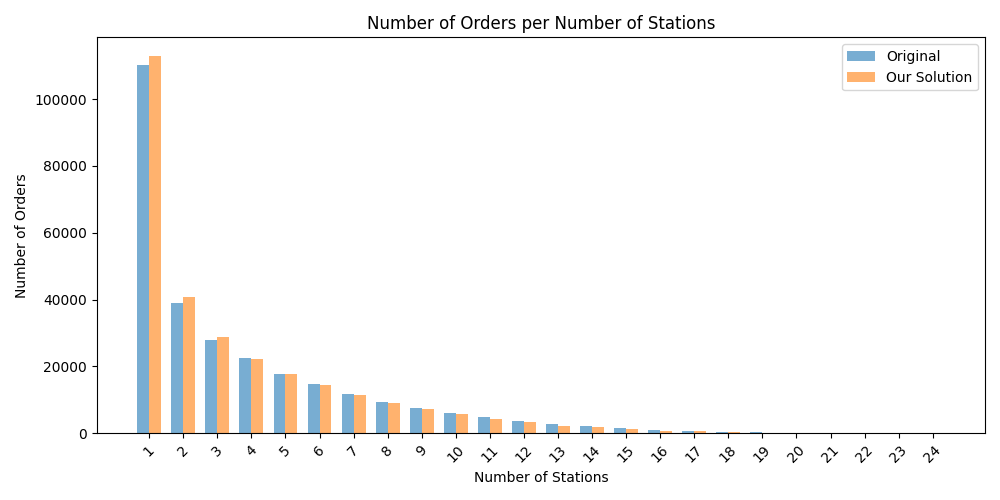
\includegraphics[width=0.85\linewidth, height=4cm]{Images_CSLAP/r4_number_of_orders_per_number_of_stations.png}
\caption{Number of Orders per Number of visited stations }
\label{fig:heuristic_orders}
\end{figure}

~\cref{fig:heuristic_orders} shows the distribution of orders by the number of visited stations. The solution provided by our heuristic approach shifts the distribution toward fewer stops: A larger share of orders visit only a small number of stations, while the incidence of orders requiring many stations declines, consistent with the objective of minimizing station visits per order.

\begin{figure}[H]
    \centering
    \begin{minipage}[b]{0.49\linewidth}
        \centering
        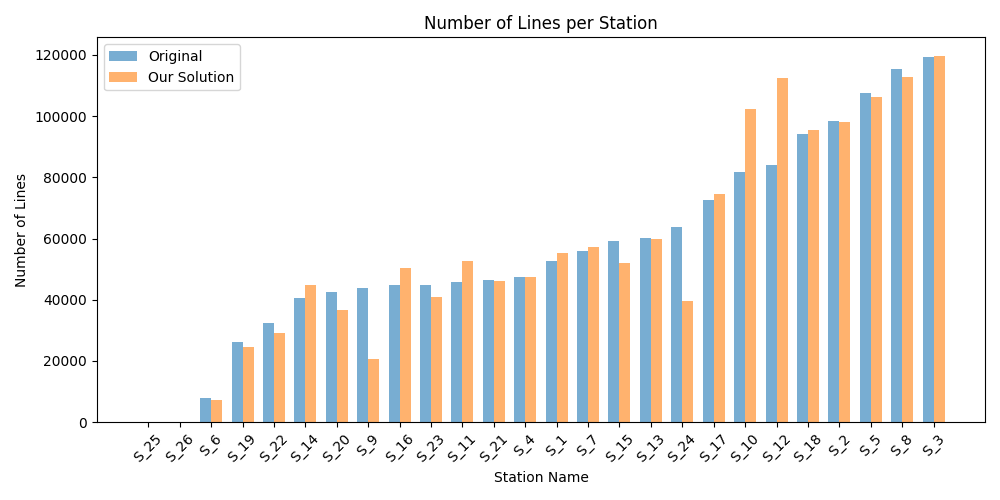
\includegraphics[width=\linewidth, height=4cm]{Images_CSLAP/r4_number_of_lines_per_station.png}
    \end{minipage}
    \hfill
    \begin{minipage}[b]{0.49\linewidth}
        \centering
        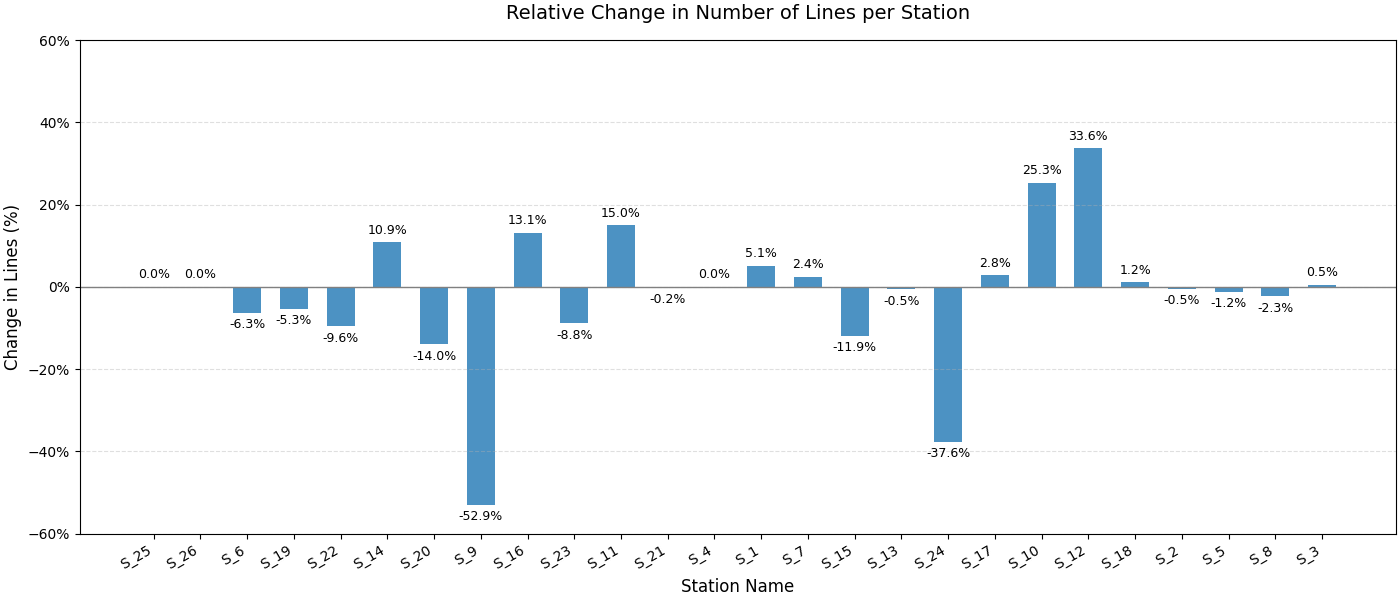
\includegraphics[width=\linewidth, height=4cm]{Images_CSLAP/r5_pct_change_lines_per_station.png}
    \end{minipage}
        \caption{Number of Lines per Station (left) and Relative Percentage Change in Lines per Station (right) from heuristic assignment, compared with the Original Assignment.}
    \label{fig:comparison_lines_heuristic}
\end{figure}

\hyperref[fig:comparison_lines_heuristic]{Figure 3} illustrates the workload distribution across stations after applying our heuristic solution. The comparison highlights that our heuristic solution effectively reduces overall station visits, although it deviates from the "balanced workload" distribution across stations that we mentioned in this \cref{par:balanced_workload}. Subject to management preferences regarding workload balancing and resource allocation flexibility, this solution can be still considered feasible in practice.


\subsection{Second Approach: Mixed-Integer Linear Programming}\label{sec:LP_Approach}

The heuristic reduces station visits quickly but can leave workloads uneven across stations.
To remedy this, we develop a Mixed-Integer Linear Programming (MILP) model that \emph{simultaneously} minimises station visits and enforces balanced workloads.

Building on the demand-correlation ideas of \cite{wang2020}, who minimize travel distance, we redirect the objective toward minimizing the \emph{number of station stops}. Orders thus flow through fewer stations, cutting queues and handling time.

The formulation employs binary decision variables (DVs) to encode product–station assignments and auxiliary variables to record, for each order, the stations it visits. The formulation ensures capacity constraints, workload balancing, and station visit counting, which is internally consistent with the corresponding product-to-station assignments.

%\noindent \textbf{Model Formulation}

\noindent \textbf{Decision variables:}
\begin{itemize}
    \item $x_{ps}$: Binary variable indicating whether product $p \in P$ is assigned to station $s \in S$.
    \item $z_{os}$: Auxiliary variable indicating whether order $o \in O$ needs to visit station $s \in S$ (completely dependent on $x_{ps}$). 

\end{itemize}

\noindent \textbf{Objective function:}

\begin{equation}
\min \sum_{o \in O} \sum_{s \in S} z_{os}
\label{obj}
\end{equation}
The objective is to minimize the total number of station visits required across all orders.

\noindent \textbf{Constraints:}

\begin{align}
&\sum_{s \in S} x_{ps} = 1 \quad \forall p \in P \label{con14}\\
&\sum_{p \in P} x_{ps} \leq \zeta_s \quad \forall s \in S \label{con15}\\
&x_{ps} \leq z_{os} \quad \forall p \in P_o, \forall o \in O, \forall s \in S \label{con16}\\
&\sum_{p \in P_o} x_{ps} \cdot \frac{L_p}{V_s} \leq T_s \quad \forall s \in S \label{con17}\\
&x_{ps} \in \{0, 1\}, \quad z_{os} \in [0,1], \quad \forall p \in P, o \in O, s \in S 
\end{align}
\\
\noindent Here, Constraint \eqref{con14} ensures each product is assigned to exactly one station, while Constraint \eqref{con15} respects the capacity limit of each station. Constraint \eqref{con16} links product assignments with station visits, and Constraint \eqref{con17} maintains a balanced workload on each station.

\subsubsection{Results on the mixed integer linear programming approach}
This section reports results from applying our linear programming model through a commercial solver like Hexaly (i.e. LocalSolver) to address the Correlated Storage Location Assignment Problem (CSLAP). Given the dataset’s scale, we have used strategic filtering such that the model remains tractable for a large real-world instance.


\subsubsection{Sub-approaches}

The complete industrial instance supplied by Company~A contains $21\,877$ Stock Keeping Units (SKUs) distributed over $26$ pick-stations.  
Solving the MILP on this full data set is infeasible within an acceptable time on any commercial solver.  
We therefore applied a frequency-based pruning scheme: In our case study, SKUs with a frequency below a certain threshold (e.g., frequency = 4) are considered stable, meaning their storage positions rarely significantly affect the overall station-visit optimization. Thus, these stable SKUs are' frozen' at their original assignments to reduce model complexity and improve computational efficiency without substantially compromising solution quality.  
%Two fringe stations with at most two locations each are also removed from the optimization instance, so every sub-approach is solved on the remaining $24$ stations.  
Although this reduction sacrifices global optimality, it yields solutions of practical quality for real-world operations. Accordingly, we tested four sub-approaches, each distinguished by specific filtering criteria and solver configurations:

\begin{itemize} 
    \item \textbf{Sub-approach~1 (Minimal Filtering):}  
          All single-item orders are removed and any SKU ordered fewer than four times is frozen.  
          The resulting model contains $16\,480$ SKUs --- \textbf{about $75\%$ of the original catalogue}.  
          No MIP start solution is supplied.

    \item \textbf{Sub-approach~2 (Minimal Filtering $+$ MIP Start):}  
          Uses the same instance as Sub-approach~1 ($16\,480$ SKUs, 24 stations) but we seed the original placement of Company A as an MIP start solution to steer the solver's initial search.

    \item \textbf{Sub-approach~3 (Elevated Filtering $+$ MIP Start):}  
          Retains only orders with more than five distinct items and freezes every SKU picked fewer than five times.  
          The resulting MILP includes $14\,416$ SKUs \textbf{around $65\%$ of the full set}.  
          The model is again initialised with the legacy assignment.

    \item \textbf{Sub-approach~4 (Elevated Filtering $+$ MIP Start, Set DV):}  
          Same data set as Sub-approach~3 but reformulated in Hexaly with \emph{set DV} rather than binary/continuous variables \cite{blaisemodeling}. In Hexaly, a set decision variable is a single high-level variable that represents an unordered subset of a finite domain. We create one such variable \( \Phi_s \) for every pick-station $s\in S$; its value is the subset of SKU indices assigned to that station. The usual binary matrix $x_{ps}$ is therefore replaced by the family \( \{\Phi_s\}_{s \in S}\), which reduces the DV to only 24 sets, and cleaner algebra with high level operations (e.g., \textit{partition},\textit{contains},\textit{count}); translate directly to increased solver efficiency.
          
\end{itemize}

All frozen SKUs (25--35\% of the total, depending on the sub-approach) remain in their original locations and continue to count towards station visits when the objective is evaluated, ensuring that the reported improvements are fully consistent with the physical warehouse. \newline
The MILP remains extremely challenging even after pruning. To keep computation within a practical window we imposed a uniform time limit of 72,000 seconds (20 h) on every run. The shown results correspond to the best solution obtained by the solver at the end of time limit.







\subsubsection{Quantitative Analysis}

\begin{table}[H]
  \centering
  \small\setlength{\tabcolsep}{4pt}
  \begin{threeparttable}

  \label{tab:MILP_comparison}

  \begin{tabularx}{\linewidth}{@{}l*{6}{>{\centering\arraybackslash}X}@{}}
    \toprule
    & \textbf{Orig.} & \textbf{Heur.} & \textbf{Sub-1} &
      \textbf{Sub-2} & \textbf{Sub-3} & \textbf{Sub-4} \\ \midrule
    Total visits     & 1\,062\,522 & 1\,013\,344 & 1\,003\,930 &
                       980\,131    & 977\,336    & 967\,133 \\
    Mean visits      & 3.730 & 3.557 & 3.524 & 3.441 & 3.431 & 3.395 \\
    Time (s)         & –     & 45    & 72\,000 & 72\,000 & 72\,000 & 72\,000 \\ \bottomrule
  \end{tabularx}
  \end{threeparttable}
    \caption{Comparison of MILP Results under Different Sub-approaches with the Original Placement and the Heuristic Algorithm-Derived Assignment}
\end{table}

Results underscore the value of providing a feasible initial solution (MIP start) and pruning low-frequency or low-impact items. Sub-approach 3 yields the strongest improvement in binary formulation, but the biggest reduction is achieved in sub-approach 4. Taken together, these two settings show that targeted data pruning can materially steer the solver toward better solutions within practical time limits.

\subsubsection{Visual Representation and Analysis for Final Results}

The following figures compare Company A’s baseline assignment with the outcomes of the final workload-balanced model (Sub-approach 4), which delivered the best reduction.


\begin{figure}[H]
\centering
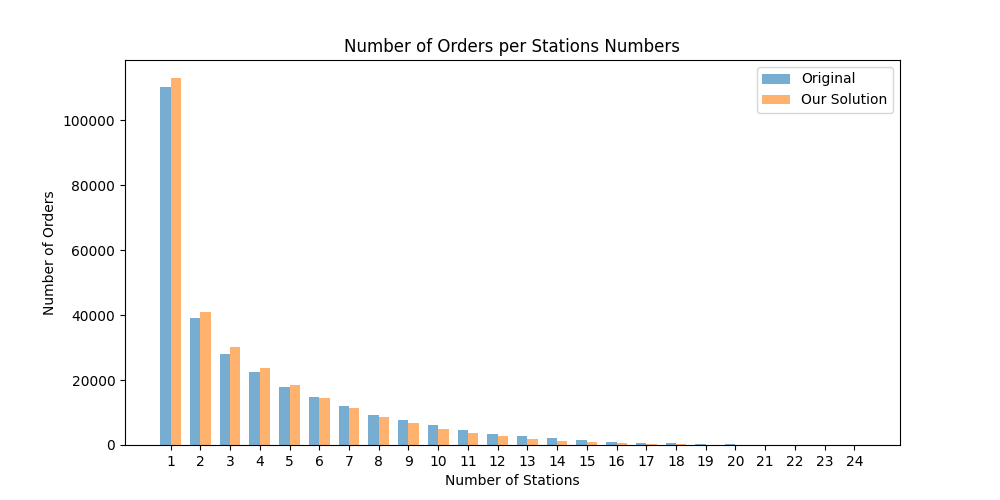
\includegraphics[width=0.85\linewidth, height=4cm]{ Images_CSLAP/Hexaly_number_of_orders_per_station_numbers (1).png}
\caption{Number of orders per number of visited stations by sub-approach 4}
\label{fig:final_orders_per_station}
\end{figure}


\hyperref[fig:final_orders_per_station]{Figure 4} shows the distribution of orders by the number of visited stations. The solver's solution shifts the mass of orders to visit only a few stations and reducing orders requiring to visit to many stations, which aligns with our objective of minimizing station visits per order.

\begin{figure}[H]
    \centering
    \begin{minipage}[b]{0.49\linewidth}
        \centering
        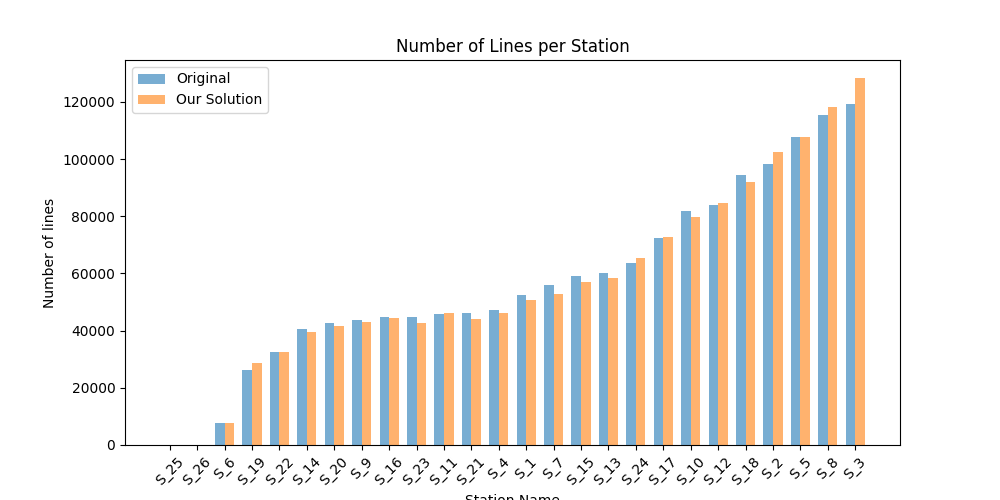
\includegraphics[width=\linewidth, height=4cm]{Images_CSLAP/Hexaly_number_of_lines_per_station.png}
    \end{minipage}
    \hfill
    \begin{minipage}[b]{0.49\linewidth}
        \centering
        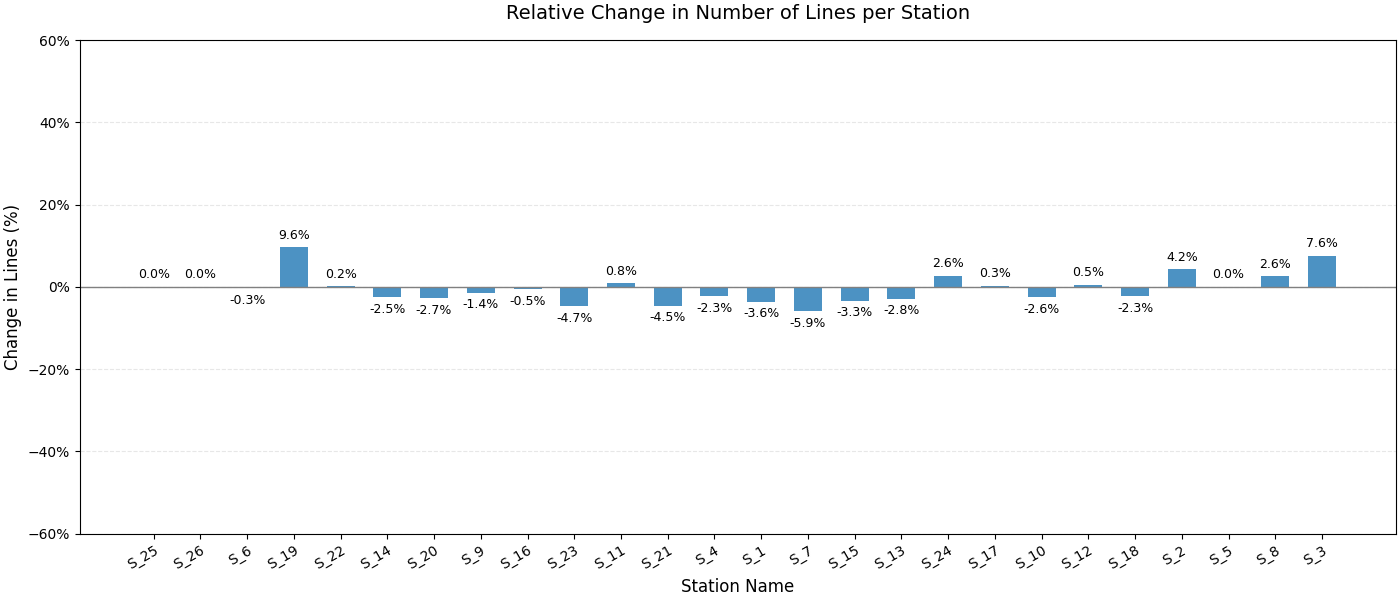
\includegraphics[width=\linewidth, height=4cm]{Images_CSLAP/Hexaly_pt_relative_change_number_of_lines_per_station.png}
    \end{minipage}
    \caption{Number of Lines per Station (left) and Relative Percentage Change in Lines per Station (right) from solver assignment (sub-approach 4), compared with the Original Assignment.}
    \label{fig:comparison_lines}
\end{figure}

\hyperref[fig:comparison_lines]{Figure 5} illustrates the workload distribution based on the assignment from the solver on sub-approach 4. It can be observed that the distribution obtained is very close to the one derived from Company A’s original placement which is the "balanced workload" we explained in this \cref{par:balanced_workload}, and the relative percentage–change on each station is substantially smaller compared to what we achieved through the heuristic solution, while at the same time, we have managed to minimize our objective.



\paragraph{\textbf{Real-World Time Savings Labor Impacts: }} The best MILP layout (Sub-approach 4) cuts about \textbf{1 444 station visits per day}, a \textbf{9 \%} drop from the original 16 098 stops/day. Over 66 working days ($\approx$ 3 months) this removes \textbf{95 304 stops}, freeing roughly \textbf{six full operating days} of picker/robot time each quarter. In practice, the site can process the same order volume almost a week faster every three months simply through better slotting.



\subsection{Robustness validation via temporal hold-out}\label{sec:temporal_validation}

To assess the robustness of decisions made from limited historical data, we evaluate layouts \emph{out of sample} by making optimized decision on early weeks and testing on later, unseen weeks. This temporal hold-out mirrors realistic deployment (optimize once, then operate as demand evolves) and is consistent with robustness practices in storage assignment and warehouse optimization where perfect information benchmarks (``oracle'' layouts) are contrasted with implementable policies \citep{lee2020cie,wang2020}. We performed two hold-out validation experiments on our 13-week dataset (3-month horizon):

\begin{itemize}
  \item \textbf{Experiment 1:} Our model makes decisions knowing only the first\,10 weeks of data, then it is evaluated on the remaining 3 weeks.  

  \item \textbf{Experiment 2:} Our model makes decisions knowing only the first\,8 weeks of data, then it is evaluated solely on the final 5 weeks.

\end{itemize}

These solutions are benchmarked against the original placement and against the “oracle” layout obtained when the MILP is optimized on the hold-out weeks.




\begin{table}[H]
\centering
\small
\renewcommand{\arraystretch}{1.15}
\setlength{\tabcolsep}{8pt}
\begin{tabular}{@{}llcc@{}}
\toprule
\textbf{Validation} & \textbf{Layout (Training Period)} & \textbf{Total Visits} & \textbf{Avg. Visits} \\
\midrule
\multirow{3}{*}{Last 3 weeks} & Baseline (Original placement) & 265,876 & 4.052 \\
& MILP (optimised on first 10 weeks) & 248,358 & 3.785 \\
& MILP Oracle (optimised on last 3 weeks) & 233,728 & 3.562 \\
\midrule
\multirow{3}{*}{Last 5 weeks} & Baseline (Original placement) & 423,593 & 3.926 \\
& MILP (optimised on first 8 weeks) & 392,318 & 3.636 \\
& MILP Oracle (optimised on last 5 weeks) & 380,356 & 3.525 \\
\bottomrule
\end{tabular}
\caption{Station-visit performance evaluated on distinct hold-out validation periods.}
\label{tab:temporal_validation}
\end{table}



\paragraph{\textbf{Discussion}}

The results of the validation experiments demonstrate the practical robustness of decisions derived from limited historical data: \\
\textbf{Experiment 1:}
Using only the first 10 weeks cuts station visits by 6.6\% versus the baseline, while the oracle, optimized directly on the test weeks, achieves 12.1\%. This gap ($\approx$5\%) shows that some short-term effects are missed, yet most of the benefit is already captured. \\
\textbf{Experiment 2:}
With eight weeks of history, the MILP reduces visits by 7.4\%; the oracle gains 10.2\%.
Again, historical correlations yield a strong but not exhaustive improvement.
Thus, for this \textit{specific warehouse}, the recent past provides guidance that is \emph{good enough for meaningful savings}, although not completely predictive. However, we acknowledge such stability might vary in different operational contexts. Hence, future work should explore incorporating predictive models or stochastic scenario planning to further manage demand uncertainties.



\subsection{Column Generation Approach}



We propose a Column Generation (CG) framework to reduce the complexity of the MILP in order to deliver high-quality solutions more quickly. CG efficiently solves combinatorial optimization problems involving vast solution spaces \cite{lubbecke2005selected}, making it ideal for set-covering and set-partitioning problems in logistics, scheduling, and warehouse management \cite{desrochers1989column}.

Set Cover and its dual, Hitting Set, are classic NP-complete combinatorial problems, require selecting minimal subsets that cover a defined universe \cite{garey1979computers}. These foundational problems underlie warehouse storage assignments and similar logistical challenges due to their structural simplicity and complexity \cite{caprara2000algorithms}.

For correlated storage assignment problems in warehouses, Set Cover naturally arises when identifying minimal item clusters covering entire orders, thus improving picking efficiency \cite{xiao2010correlated}. CG effectively solves such problems by iteratively refining solutions through a master and a pricing subproblem \cite{lubbecke2005selected}. Our CG implementation iteratively generates feasible product-station assignment patterns (columns) based on dual variable values, significantly enhancing computational efficiency compared to exhaustive enumeration.


\subsubsection{Framework Overview}

To keep the master problem tractable, we adopt a strategy where product assignment patterns are generated independently for each station. This localized generation of feasible assignments reduces the dimensionality of the master problem, as it no longer needs to enforce product assignment uniqueness across all stations during each iteration. Instead, a diverse set of candidate patterns is generated dynamically, guided by the dual variables obtained from the master problem.




\subsubsection{Master Problem Formulation}

The master problem aims to select the optimal combination of station assignment patterns that collectively minimize the total number of visited stations required to fulfill all orders. The formulation ensures that:

\begin{itemize}
    \item Each product is assigned to exactly one station (uniqueness of assignment).
    \item The total workload at each station does not exceed its capacity.
    \item Only one assignment pattern is selected for each station.
\end{itemize}


\paragraph{Parameters:}
\begin{itemize}
    \item $\delta_{psk}$: Binary parameter equal to 1 if product $p$ is included in pattern $k$ for station $s$, 0 otherwise.
    \item $z_{osk}$: Binary parameter equal to 1 if any product from order $o$ is included in pattern $k$ for station $s$, 0 otherwise.
\end{itemize}

\paragraph{Standing assumptions:}
(i) Every feasible pricing pattern respects the station capacity, (i.e.,
\(
\sum_{p\in P}\delta_{psk}\ \le\ \zeta_s \qquad \forall s\in S,\ \forall k\in K_s,
\))
and (ii) the total capacity equals the number of products:
\(
\sum_{s\in S}\zeta_s\ =\ |P|.
\)


\paragraph{Decision variables:}
\begin{itemize}
    \item $y_{sk} \in \{0,1\}$: 1 if pattern $k$ is selected for station $s$, 0 otherwise.
   
\end{itemize}



\paragraph{Objective function:}
Minimize the total number of visited stations required across all orders:
\[
\min \sum_{o \in O} \sum_{s \in S} \sum_{k \in K_s} z_{osk} \cdot y_{sk}
\]

\paragraph{Constraints:}
\begin{enumerate}
    \item \textbf{Pattern selection constraint:} Ensure that at most one pattern is selected for each station.
    \[
    \sum_{k \in K_s} y_{sk} \leq 1 \quad \forall s \in S \quad \quad \quad \quad \quad (\pi_s)
    \]

    \item \textbf{Product assignment constraint:} Ensure that the universe of products is included, and since the above constraint will assure the selection of only one pattern per station (along with assumptions we gave), this constraint will then make sure that the patterns selected for each station in the end will be unique and so each product will be assigned in exactly one station.
    \[
    \sum_{s \in S} \sum_{k \in K_s} \delta_{psk} \cdot y_{sk} \geq 1 \quad \forall p \in P\quad \quad \quad \quad (\sigma_{p})
    \]

    \item \textbf{Variable domains:}
    \[
    y_{sk} \in \{0,1\} \quad \forall s \in S, \forall k \in K_s
    \]
\end{enumerate}

 The master problem is solved iteratively with an initial feasible set of patterns, and it will supply the pricing problem with these dual coefficients: ($\pi_s$) for pattern selection and ($\sigma_p$) for product coverage. As the solution progresses, new patterns with the potential to improve the objective value are introduced through the pricing problem.




\subsubsection{Pricing Problem}
The pricing problem is tasked with generating new station assignment patterns by solving a subproblem for each station. These subproblems leverage the dual values obtained from the master problem to identify assignments that can reduce the overall cost (i.e., station visits). If any new pattern has a negative reduced cost, it is added to the master problem for further optimization. This iterative process continues until no new pattern with negative reduced costs can be generated, indicating optimality with respect to the current formulation.

\paragraph{Decision variable:}
\begin{itemize}
    \item $x_p \in \{0,1\}$: 1 if product $p$ is included in the new pattern at station $s$, 0 otherwise.
    \item $z_o \in \{0,1\}$: 1 if order $o$ requires visiting station $s$ due to the new pattern, 0 otherwise. it is dependent on $x_p$
\end{itemize}
 

\paragraph{Objective function:}
Minimize the reduced cost:
\[
\min \left\{ \sum_{o \in O} z_o - \sum_{p \in P} \sigma_{p} x_p \right\}
+ \pi_s\]

\paragraph{Constraints:}
\begin{enumerate}
    \item \textbf{Order inclusion constraints:} Ensure that $z_o$ is set to 1 if any product from order $o$ is included in the pattern.
    \[
    z_o \geq x_p \quad \forall o \in O, \forall p \in P_o
    \]

    \item \textbf{Capacity constraint:} The total number of products assigned to station $s$ does not exceed its capacity.
    \[
    \sum_{p \in P} x_p \leq \zeta_s
    \]

    \item \textbf{Workload constraint:} The total workload of the pattern must not exceed the station's capacity.
    \[
    \sum_{p \in P} x_p \cdot \frac{L_p}{V_s} \leq T_s
    \]

    \item \textbf{Variable domains:}
    \[
    x_p \in \{0,1\} \quad \forall p \in P
    \]
    \[
    z_o \in [0,1] \quad \forall o \in O
    \]
\end{enumerate}


\subsubsection{Final Optimization Step}\label{par:final_optimization_step}



Upon convergence, CG yields fractional solutions requiring a final discrete assignment step. We resolve the master problem once more, enforcing binary decisions to ensure a precise assignment that meets practical warehouse constraints, product assignment uniqueness, balanced workloads, and minimal station visits.

Although accurate, this exact approach can be computationally intensive for large datasets. Future research could explore alternative post-processing techniques, such as rounding heuristics (quick approximations prioritizing feasibility), hybrid heuristic-exact methods (heuristics refined by limited exact optimization), and metaheuristic methods (genetic algorithms, tabu search, simulated annealing), which strategically search solution spaces to balance computational efficiency and solution quality for practical warehouse settings.



\subsubsection{Results on the column generation approach}

In this subsection, we present numerical results obtained from the implementation of our proposed CG approach and provide a comparative evaluation against the previously discussed Heuristic and MILP approaches. Due to the complex structure of our CG formulation, consisting of a single master problem and multiple pricing problems (one for each station), achieving global optimal solutions becomes computationally prohibitive when dealing with the large-scale real-world dataset in its entirety. To effectively illustrate the merits of the CG method, we conduct our experiments on two representative subsets of the original dataset. This approach highlights the significant advantages of CG when applied to smaller datasets than typical real-world scenarios, but aligning with the scale commonly adopted in existing literature to validate theoretical aspects of optimization methodologies.

Specifically, we consider two distinct scenarios differing in scale and complexity:

\begin{itemize} \item \textbf{Scenario 1:} 25 Products, 601 Orders, and 11 Stations. \item \textbf{Scenario 2:} 46 Products, 3497 Orders, and 13 Stations. \end{itemize}

These scenarios are selected to provide insights into how the CG approach (solved using CPLEX) compares in terms of solution optimality and computational performance relative to the Heuristic and MILP (solved using Hexaly) under the sub-approach 4 conditions. The objective is to highlight the potential benefits of our CG approach in smaller-scale contexts, thus validating its applicability and efficiency as part of a multi-method optimization framework for the Correlated Storage Location Assignment Problem (CSLAP).



\subsubsection{Quantitative Analysis First Scenario}


\begin{table}[H]
  \centering
  \small\setlength{\tabcolsep}{4pt}
  \begin{threeparttable}
  \begin{tabularx}{\linewidth}{@{}l*{4}{>{\centering\arraybackslash}X}@{}}
    \toprule
    & \textbf{Orig.} & \textbf{Heur.} & \textbf{MILP} & \textbf{CG} \\ \midrule
    Total number of visits     & 1\,209 & 1\,094 & 1\,097 & 1\,097 \\
    Mean number of  visits      & 2.012 & 1.820 & 1.825 & 1.825 \\
    Computation Time (s)         & –     & 2     & 377   & 80    \\ \bottomrule
  \end{tabularx}
  \end{threeparttable}
  \caption{Comparison of CG Results under first scenario dataset with the MILP under sub-approach 4 conditions, Heuristic and Original Placement}
\label{tab:CG_25_comparison}

\end{table}



The results presented on \hyperref[tab:CG_25_comparison]{Table 7} show that the heuristic solution achieves the lowest total number of station visits and thus the greatest apparent reduction in our primary objective, but this approach lacks practical applicability because it is limited due to not considering a constraint to maintain a balanced workload across stations. Conversely, both the MILP and the CG attain the global optimal solution regarding station visits, while maintaining a good workload distribution. However, a key advantage of the CG approach is evident in its computational performance; it achieves the same optimal solution as MILP but with much faster computation time.



\subsubsection{Visual Representation and Analysis for First Scenario}


\textbf{Number of  Lines Per Station:}
This analysis compares the workload distribution, measured by the number of retrieval lines, across each station for all evaluated approaches (Original, MILP, CG, and Heuristic) under Scenario 1. The dashed lines labeled \emph{Optimal} represent the reference workload distribution initially established by Company A as ideal, as previously explained in this section on the Case Study~\cref{par:balanced_workload}.

\begin{figure}[H]
    \centering
    \begin{minipage}[b]{0.49\linewidth}
        \centering
        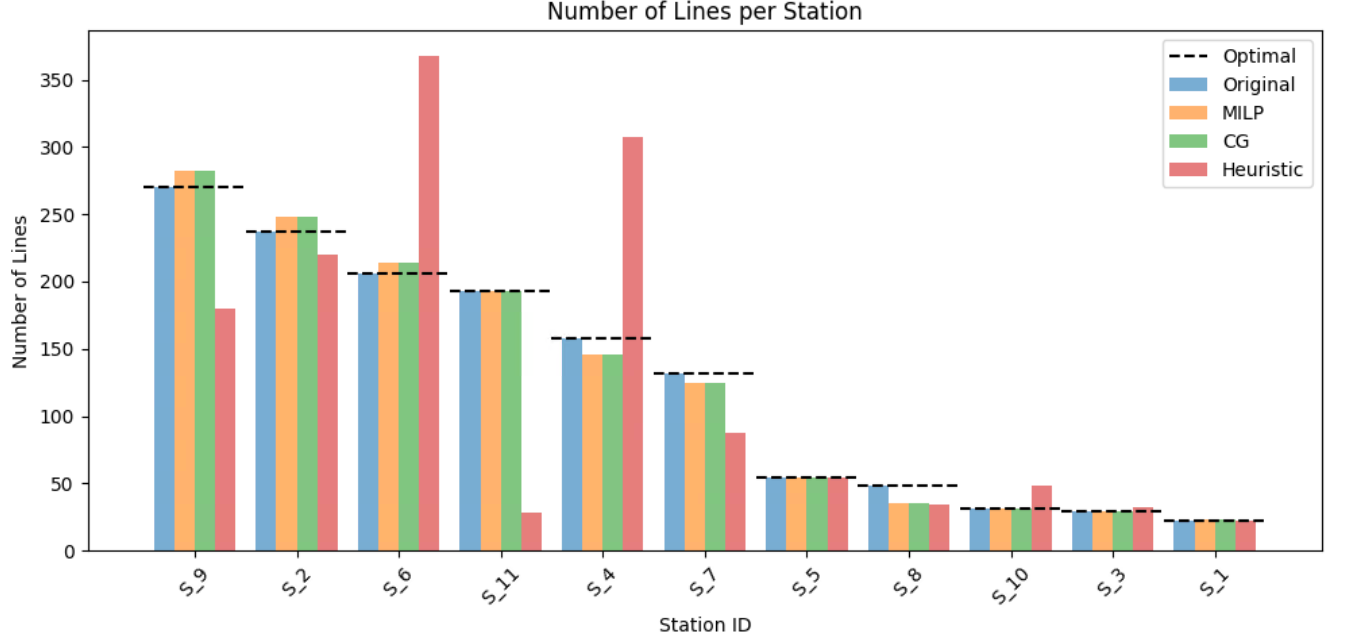
\includegraphics[width=\linewidth, height=4cm]{Images_CSLAP/Number_Lines_CG_25.png}
    \end{minipage}
    \hfill
    \begin{minipage}[b]{0.49\linewidth}
        \centering
        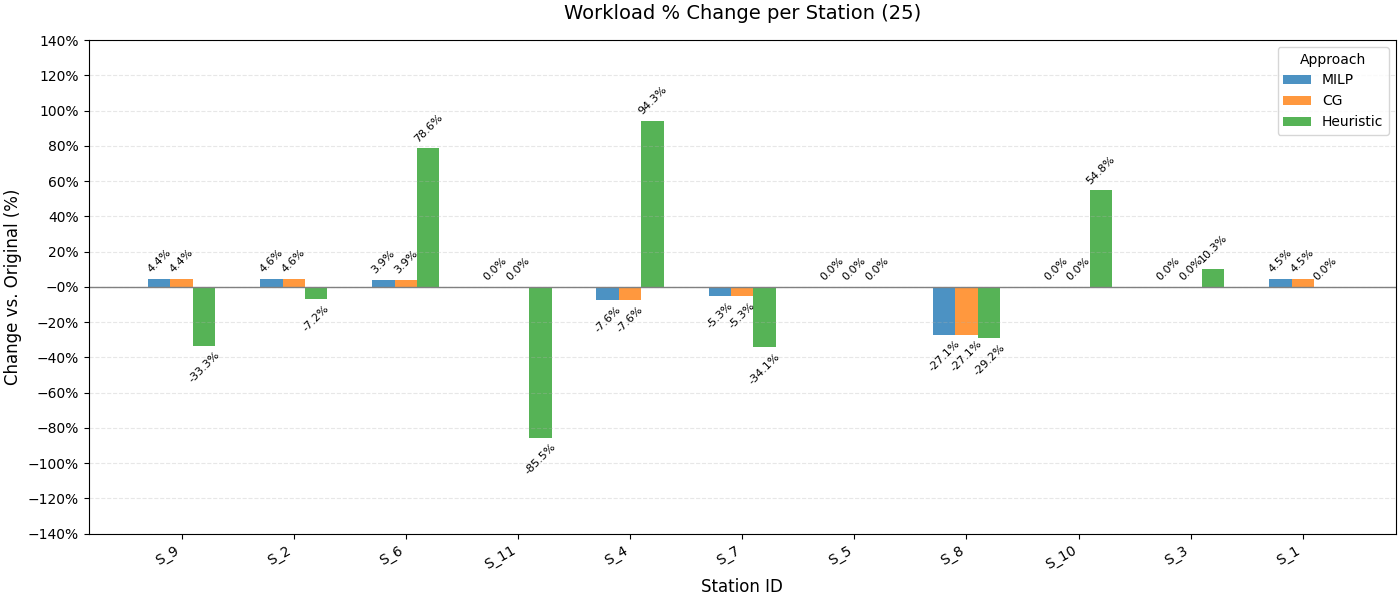
\includegraphics[width=\linewidth, height=4cm]{Images_CSLAP/25_workload_pct_change.png}
    \end{minipage}
        \caption{Number of Lines at each Station (left) and Relative Percentage Change in Lines per Station (right) based on Scenario 1.}
\end{figure}

The MILP and CG solutions yield distributions that closely track Company A’s baseline (dashed lines) while still reducing the objective. On the other hand, we check that our heuristic can achieve a great reduction in our objective, but it does not preserve a well-balanced workload in the warehouse \cref{par:balanced_workload}.


\subsubsection{Quantitative Analysis Second Scenario}


\begin{table}[H]
  \centering
  \small\setlength{\tabcolsep}{4pt}
  \begin{threeparttable}



  \begin{tabularx}{\linewidth}{@{}l*{4}{>{\centering\arraybackslash}X}@{}}
    \toprule
    & \textbf{Orig.} & \textbf{Heur.} & \textbf{MILP} & \textbf{CG} \\ \midrule
    Total number of visits     & 8\,589 & 7\,444 & 7\,458 & 7\,410 \\
    Mean number of visits      & 2.456 & 2.129 & 2.133 & 2.119 \\
    Computation Time (s)         & –     & 3     & 50\,000 & 3\,258 \\ \bottomrule
  \end{tabularx}
  \end{threeparttable}
    \caption{Comparison of CG Results under second scenario dataset with the MILP under sub-approach 4 conditions, Heuristic and Original Placement}
    \label{tab:CG_46_comparison}
\end{table}
The results presented on \hyperref[tab:CG_46_comparison]{Table 9} highlight notable differences among the evaluated methods. The heuristic solution achieves a significant reduction in our primary objective, but its practical applicability is again limited due to its inability to maintain a balanced workload across stations. The MILP approach attains a good quality reduction in our objective while maintaining a good workload distribution, but we see that the computation time is very high. On the CG approach, the results show that we reach the highest minimum for our objective, and the key advantage is its computational performance, where we achieve better results than the MILP approach in a fraction of the computation time. 

\subsubsection{Visual Representation and Analysis for Second Scenario}


\textbf{Number of  Lines Per Station:}
As before now we present the workload distribution across stations for Scenario 2, measured by the total number of retrieval lines. 
%As previously defined, the dashed lines labeled \emph{Optimal} correspond to the ideal station workloads established by Company A (Section~\ref{par:balanced_workload})

\begin{figure}[H]
    \centering
    \begin{minipage}[b]{0.49\linewidth}
        \centering
        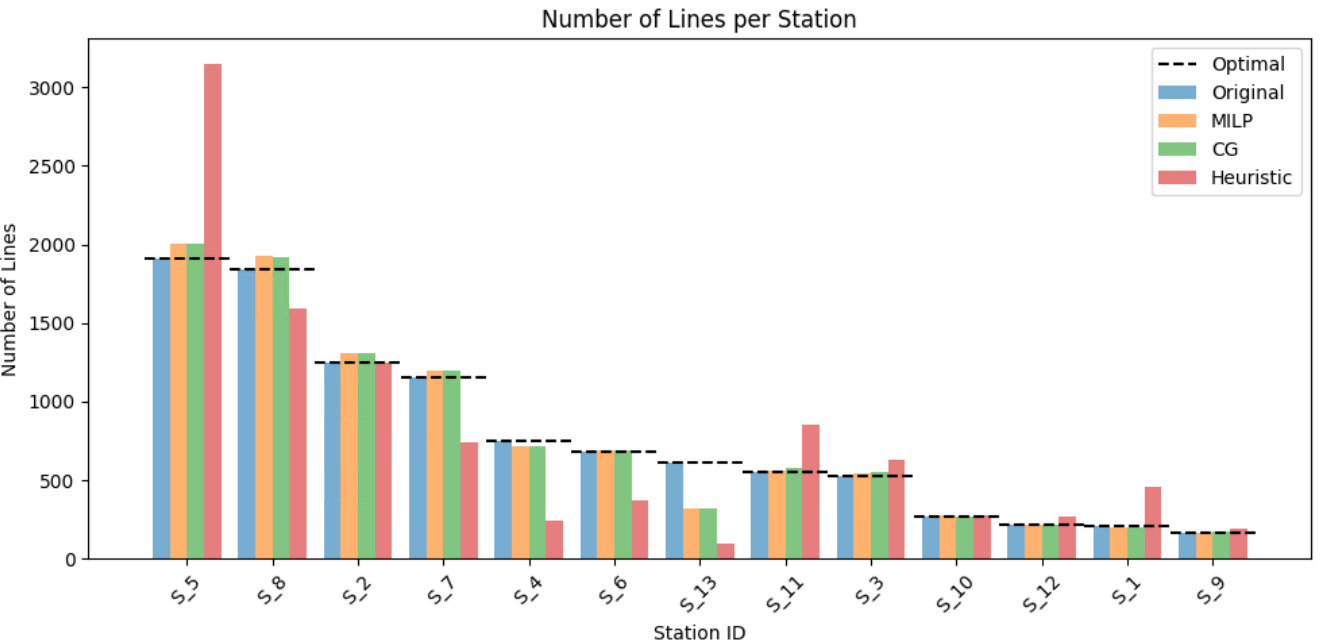
\includegraphics[width=\linewidth, height=4cm]{Images_CSLAP/Number_Lines_CG_46.png}
    \end{minipage}
    \hfill
    \begin{minipage}[b]{0.49\linewidth}
        \centering
        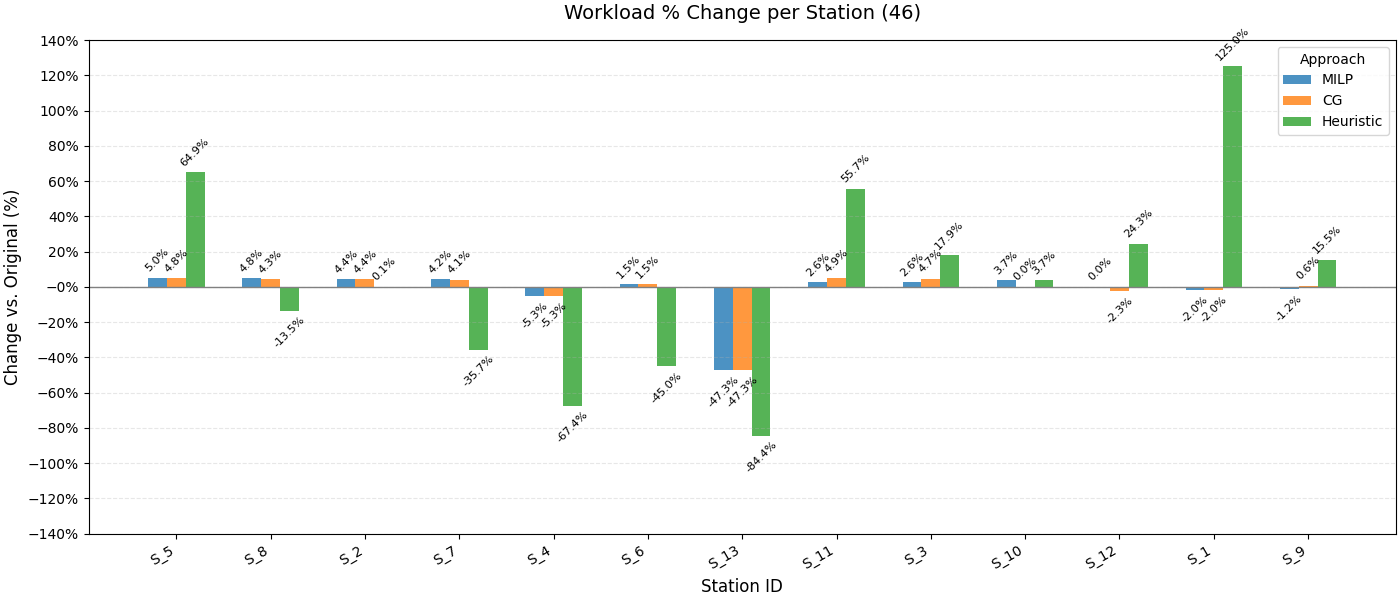
\includegraphics[width=\linewidth, height=4cm]{Images_CSLAP/46_workload_pct_change.png}
    \end{minipage}
        \caption{Number of Lines at each Station (left) and Relative Percentage Change in Lines per Station (right) based on Scenario 2.}
\end{figure}

For Scenario 2, both the MILP and CG approaches again closely approximate the optimal workload distribution, demonstrating consistency in their ability to balance station workloads effectively across larger and more complex datasets. 


\noindent
These experiments showed that CG matches the MILP optimum in a fraction of the time, making it the best trade-off between quality and speed in our study. The MILP approach similarly achieves high-quality solutions, but with less computational efficiency than CG, while the heuristic is fastest yet sacrifices workload balance. \\
\emph{\textbf{As a preliminary step toward scaling CG to the full industrial instance,}} we also tested a fast heuristic pricing scheme (greedy workload-based station sequencing and fixed-size patterns built from dual lift, cohesion score based on first heuristic \cref{alg:greedy-cslap} and popularity based on product frequency). Although it routinely produced negative reduced-cost columns, it under-accounted for cross-station workload coupling and tended to concentrate high-lift products on a single station. Consequently, the master either violated workload targets or lost most gains during re-balancing. We therefore report results with exact pricing and view this heuristic variant as an initial probe to guide scalable enhancements. \\
Because our validation is still on limited-scale subsets, future work will investigate advanced CG enhancements (e.g., stronger pricing heuristics with explicit workload penalties, stabilization, parallelization, and alternative post-processing techniques \cref{par:final_optimization_step}) to extend the same efficiency gains to the full-size CSLAP instances of our case study.


\subsection{\textbf{Remark: Real-World Implementation with Limited Product Reassignment}}
\label{sec:limited_reassignment}

\noindent

While the Linear Programming (LP) model described in \cref{sec:LP_Approach} provides a pathway to minimize station visits and balance workloads, fully redesigning storage assignments can be impractical in an operational warehouse. In many real-world scenarios, reassigning a large portion of products to new stations is both costly and disruptive. Moving every product to its mathematically “optimal” position may require extended downtime and significant labor, risking delays in fulfilling customer orders.

To address this concern, we introduce a practical extension that restricts the total number of products allowed to be relocated. Specifically, we limit the number of reassigned products to at most \(k\), where \(k\) is chosen according to workforce availability, downtime constraints, or a targeted percentage of total products. By doing so, we retain the advantages of the LP formulation while mitigating its impact on everyday operations.

\subsubsection{Mathematical Formulation with Limited Reassignment}
Let \(s'(p)\) denote the \emph{original} station assignment of product \(p\). In addition to the DV and constraints from \cref{sec:LP_Approach}, we add the following constraint:

\begin{equation}
\sum_{p \in P} x_{ps'(p)} \;\;\ge\;\; |P| - k, \quad \forall s' \in S,
\label{constraint:reassignment}
\end{equation}
where:
\begin{itemize}
    \item \(x_{p,\,s'(p)}\) is the original binary variable from our LP model, here used to indicate whether product \(p\) remains in its original station \(s'(p)\).
\end{itemize}

Constraint~\eqref{constraint:reassignment} enforces that at least \(|P| - k\) products must remain in their original stations, thereby limiting the number of relocated products to at most \(k\). This ensures that, although the overall objective (cf. Objective~\eqref{obj}) aims to minimize station visits, it does so within a practical cap on how many products can be moved.

\subsubsection{Results on the Restricted Mixed Integer Linear Programming Approach}
We now present the results of incorporating the limited reassignment constraint into our LP model. The same conditions used in Sub-approach~4 of \cref{sec:LP_Approach} apply here, and the problem is again solved through the Hexaly commercial solver. In this scenario, we set \(k = 500\), which corresponds to approximately \(2.2\%\) of the total products.

\subsubsection{\textbf{Quantitative Analysis}}
As before, the problem remains computationally intensive; hence, we specify a computation time limit (here, \(72{,}000\) seconds) and retain the best solution found by the solver up to that threshold.

\begin{table}[H]
  \centering
  \small\setlength{\tabcolsep}{6pt}
  \begin{threeparttable}
  \label{tab:restricted_MILP}

  \begin{tabularx}{\linewidth}{@{}l >{\centering\arraybackslash}X >{\centering\arraybackslash}X@{}}
    \toprule
    & \textbf{Original} & \textbf{Restricted MILP} \\ \midrule
    No.\ of station visits & 1\,062\,522 & 1\,060\,606 \\
    Mean visits per order  & 3.730 & 3.723 \\
    computation time (s)   & –     & 72\,000 \\ \bottomrule
  \end{tabularx}
  \end{threeparttable}
    \caption{Restricted MILP ($\leq$500 re-assignments) versus original}
\end{table}

As illustrated above the Restricted MILP approach still achieves a reduction of approximately 2{,}000 total station visits compared with the original layout, even though only about \(2.2\%\) of products are permitted to move.
Thus, capping re-slotting effort lets managers capture most of the station-visit benefit without disruptive full-scale reassignments. By selecting an appropriate limit $k$ to match labor, budget, and downtime constraints, warehouses can implement step-wise, “continuous-improvement” upgrades that raise throughput while leaving the vast majority of products undisturbed.

\section{Conclusion}
\label{sec:conclusion}

In this study, we tackled the Correlated Storage Location Assignment Problem (CSLAP) with a unique focus on minimizing station visits in automated warehouses. We evaluated three optimization methods:
\begin{itemize}
    \item \textbf{Heuristic Approach:} A greedy clustering algorithm rapidly groups frequently co-ordered products, significantly reducing station visits. Although fast and scalable, it lacks to preserve a balanced workload, potentially creating uneven workloads.
    \item \textbf{Mixed Integer Linear Programming (MILP):} Our MILP formulation precisely controls workload distribution while minimizing station visits. However, computational complexity limits its scalability, requiring strategic data filtering or heuristic starts for large, real-world problems.
    \item \textbf{Column Generation (CG):} The CG framework decomposes the problem, iteratively refining the solution with promising assignment patterns. While maintaining balanced workloads and achieving solutions faster than MILP, it still faces complexity at very large scales.
\end{itemize}

Recognizing real-world constraints, we also introduced a practical MILP extension limiting product reassignment. This approach minimizes operational disruptions by incrementally improving warehouse layouts. Our results demonstrate substantial operational improvements (a 9\% reduction or 1\,444 fewer station stops daily), highlighting the practical benefit of minimizing station visits. 

\subsection*{Managerial implications: What should operations leaders do?}

\begin{itemize}
    \item \textbf{Adopt station-visit as a KPI for slotting.} In conveyor/zone systems, station stops directly create queuing and handling delays. Track ``stops per order'' alongside travel time to reveal congestion hot spots that distance-only metrics miss.
    \item \textbf{Implement low-disruption re-slotting.} When seasonal surges or congestion dominate, use the \emph{limited-reassignment} MILP to cap moves (e.g., limited scattering of a few top SKUs \citep{liu2023scattered}, $k{=}500$ SKUs $\approx$ 2.2\%). This captures a sizable share of benefits (about $2\,000$ fewer stops in our case) while minimizing downtime and labor.
    \item \textbf{Prioritize high-impact SKU communities.} Start with communities identified by the greedy heuristic, then refine with MILP/CG under workload-balance targets to avoid creating over/under-utilized stations.
    \item \textbf{Recalibrate quarterly with rolling history.} The temporal hold-out analysis (Section~\ref{sec:temporal_validation}) shows that layouts optimized on the recent 8-10 weeks generalize well to the next 3-5 weeks. Re-optimizing on a rolling window maintains performance with limited engineering effort.
\end{itemize}

%Warehouse managers can thus strategically choose among these methods, heuristic for speed and scale, MILP or CG for balanced accuracy, and limited reassignment for operational feasibility, achieving significant efficiency gains tailored to specific operational needs.

\section {Future Research Directions}
Future work can enhance the realism of CSLAP solutions by incorporating heterogeneous product dimensions and storage constraints. Exploring hybrid clustering methods combining product attributes with frequency correlations can further optimize storage assignments. Additionally, discrete-event simulations comparing original and optimized warehouse configurations will quantitatively validate our methods, highlighting operational bottlenecks, queue dynamics, and throughput improvements. 
Further research should integrate stochastic demand patterns and robust optimization to address uncertainty in order volumes. Real-time adaptation using machine learning could dynamically refine product placements, ensuring resilient, high-performance warehouse operations in evolving supply chain contexts.




% % --------------------- Declarations & statements ------------
% \section*{Credit authorship contribution statement}

% \textbf{Ermal Belul}: Conceptualization, Methodology, Software, Data curation, Investigation, Formal analysis, Visualization, Project administration, Writing – original draft, Writing – review \& editing. 
% \textbf{Marwane Bouznif}: Conceptualization, Supervision, Validation, Writing – review \& editing.  
% \textbf{Dritan Nace}: Conceptualization, Supervision, Validation, Writing – review \& editing.  
% \textbf{Antoine Jouglet}: Conceptualization, Supervision, Validation, Writing – review \& editing.

% \section*{Acknowledgments}
% This research was carried out with the support of the Association Nationale de la Recherche et de la Technologie (ANRT), Savoye, and the University of Technology of Compiègne.

% \section*{Declaration of competing interest}
% The authors declare that they have no known competing financial interests or personal relationships that could have appeared to influence the work reported in this paper.

\begin{thebibliography}{00}

\bibitem[(Ansari and Smith, 2020)]{ansari2020}
Ansari, M., Smith, J.S., 2020. Gravity clustering: A correlated storage location assignment problem approach. In: Proceedings of the 2020 Winter Simulation Conference, 1288-1299.

% \bibitem[(Belul et al., 2025)]{ErmalBelul2025}
% Belul, E., Bouznif, M., Nace, D., Jouglet, A., 2025. Optimizing Automated Warehouse Operations: A Novel Approach to the Correlated Storage Location Assignment Problem (CSLAP), 20th Annual System of Systems Engineering Conference (SoSE), Tirana, Albania, 2025

\bibitem[(Blaise, Hexaly)]{blaisemodeling}
Blaise, L., n.d. Modeling scheduling problems with Hexaly. Hexaly, 251 Boulevard Pereire, 75017 Paris, France.

\bibitem[(Caprara et al.,2000)]{caprara2000algorithms}
Caprara, A., Fischetti, M., Toth, P., 2000. Algorithms for the set covering problem. Annals of Operations Research 98(1-4), 353-371.

\bibitem[(Chabot et al.,2024)]{chabot2024reassignment}
Chabot, T., et al., 2024. Reassignment problem. In: Warehousing and Material Handling Systems for the Digital Industry, p.~137.

\bibitem[(Desrochers and Soumis, 1989)]{desrochers1989column}
Desrochers, M., Soumis, F., 1989. A column generation approach to the urban transit crew scheduling problem. Transportation Science 23(1), 1-13.

\bibitem[(Egas and Masel, 2010)]{Egas2010-zb}
Egas, C., Masel, D., 2010. Determining warehouse storage location assignments using clustering analysis. In: Proceedings of the 11th IMHRC, Milwaukee, WI.

\bibitem[(Garey and Johnson, 1979)]{garey1979computers}
Garey, M.R., Johnson, D.S., 1979. \textit{Computers and Intractability: A Guide to the Theory of NP-Completeness}. W. H. Freeman.

\bibitem[(Islam and Uddin, 2023)]{islam2023}
Islam, M.S., Uddin, M.K., 2023. Correlated storage assignment approach in warehouses: A systematic literature review. Journal of Industrial Engineering and Management 16(2), 294--318.

\bibitem[Lee et al.(2020)]{lee2020cie}
Lee, I.G., Chung, S.H., Yoon, S.W. (2020).
Two-stage storage assignment to minimize travel time and congestion for warehouse order picking operations.
\textit{Computers \& Industrial Engineering}, 139, 106129.
%https://doi.org/10.1016/j.cie.2019.106129

\bibitem[Liu and Poh(2023)]{liu2023scattered}
Liu, M., Poh, K.L. (2023).
E-commerce warehousing: An efficient scattered storage assignment algorithm with bulky locations.
\textit{Computers \& Industrial Engineering}, 181, 109236.
%https://doi.org/10.1016/j.cie.2023.109236

\bibitem[(L{\"u}bbecke and Desrosiers , 2005)]{lubbecke2005selected}
L{\"u}bbecke, M.E., Desrosiers, J., 2005. Selected topics in column generation.
\textit{Operations Research} 53(6), 1007-1023. 
%https://doi.org/10.1287/opre.1050.0234

\bibitem[(Pang and Chan, 2016)]{pang2016}
Pang, K.-W., Chan, H.-L., 2016. Data-mining-based algorithm for storage location assignment in a randomised warehouse. International Journal of Production Research 55(14), 4035-4052.


\bibitem[(Trindade et al., 2022)]{trindade2022}
Trindade, M.A.M., Sousa, P.S.A., Moreira, M.R.A., 2022. Ramping up a heuristic procedure for the storage location assignment problem with precedence constraints. Flexible Services and Manufacturing Journal 34(3), 646-669.

\bibitem[(Wang et al., 2020)]{wang2020}
Wang, M., Zhang, R.-Q., Fan, K., 2020. Improving order-picking operation through efficient storage location assignment: A new approach. \textit{Computers \& Industrial Engineering}, 139, 106186.
%https://doi.org/10.1016/j.cie.2019.106186

\bibitem[(West et al., 2001)]{west2001introduction}
West, D.B., et al., 2001. \textit{Introduction to Graph Theory} (Vol. 2). Prentice Hall.

\bibitem[(Xiao and Zheng, 2010)]{xiao2010correlated}
Xiao, J., Zheng, L., 2010. A correlated storage location assignment problem in a single-block multi-aisle warehouse considering bill-of-material information. International Journal of Production Research 48(5), 1321--1338.

\bibitem[(Xie and Otten, 2024)]{xie2024combi}
Xie, L., Otten, S., 2024. Introducing combi-stations in robotic mobile fulfilment systems: A queueing-theory-based efficiency analysis. In: International Conference on Computational Logistics. Springer.

\bibitem[Zhang et al.(2019)]{zhang2019cie}
Zhang, R.-Q., Wang, M., Pan, X. (2019).
New model of the storage location assignment problem considering demand correlation pattern.
\textit{Computers \& Industrial Engineering}, 129, 210-219.
%https://doi.org/10.1016/j.cie.2019.01.027


\bibitem[Zhang et al.(2023)]{zhang2023rmfs}
Zhang, J., Zhang, N., Tian, L., Zhou, Z., Wang, P. (2023).
Robots’ picking efficiency and pickers’ energy expenditure: The item storage assignment policy in robotic mobile fulfillment system.
\textit{Computers \& Industrial Engineering}, 176, 108918.
%https://doi.org/10.1016/j.cie.2022.108918




\end{thebibliography}



\end{document}